\documentclass{beamer}
\usetheme{Warsaw}
%\usetheme{Frankfurt}

\usepackage[utf8]{inputenc}   
\usepackage[T1]{fontenc}      
\usepackage[francais]{babel}  

\usepackage{url}
\usepackage{listings}

\usepackage{graphicx}
\usepackage[marginpar]{todo}

\usepackage{stmaryrd}

\usepackage{pacman}

\title{Extension du langage Pythran pour le module itertools}           
\author{Alan Raynaud}
\date{}                      

\begin{document}

\lstset{language=python, numbers=left, numberstyle=\tiny,
  showstringspaces=false, frame=leftline }

\begin{frame}{Introduction}
  \titlepage
\end{frame}

\AtBeginSection[] {
  \begin{frame}<beamer> \frametitle{Plan de la présentation}
    \tableofcontents[currentsection]
  \end{frame}
}
\AtBeginSubsection[] {
  \begin{frame}<beamer> \frametitle{Plan de la présentation}
    \tableofcontents[currentsection,currentsubsection]
  \end{frame}
}

\begin{frame}{Plan de la présentation}

  \setcounter{tocdepth}{1}
  \tableofcontents
  \setcounter{tocdepth}{3}

\end{frame}

\section{Contexte}

\subsection{Python et la performance}

\begin{frame}{Performances de python}

  Python :
  \begin{itemize}
    \item Langage interprété 
    \item Dynamiquement typé
  \end{itemize}

  \pause Python est la plupart du temps moins performant que des
  langages comme C/C++.

\end{frame}

\begin{frame}{Comparaison de performances\cite{PythonVsCpp}}

  \begin{figure}[h]
    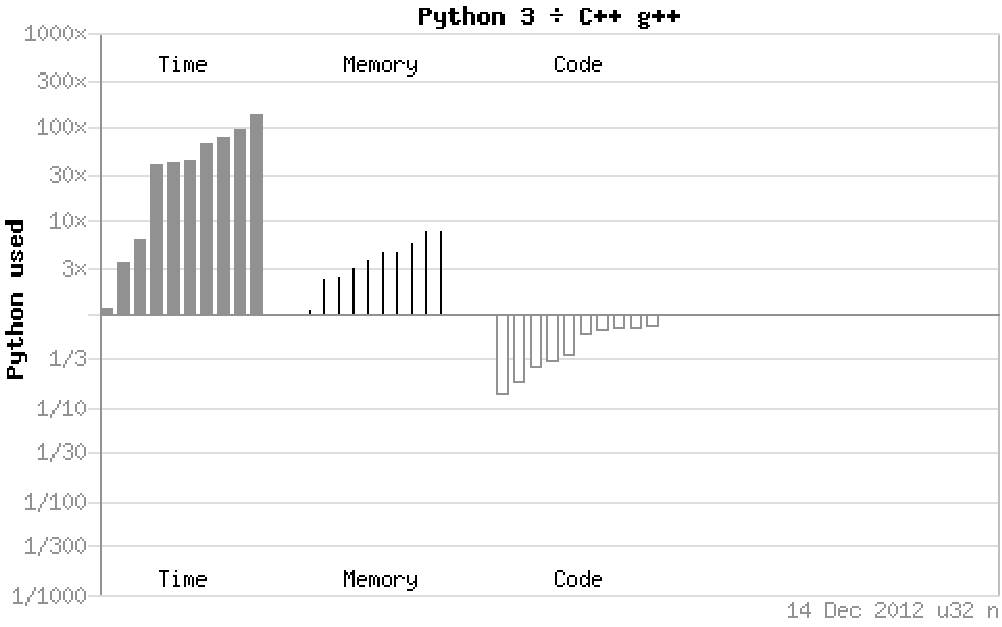
\includegraphics[width=\textwidth]{./Pictures/pythonvscpp}
    \label{pythonvscpp}
  \end{figure}

\end{frame}

\begin{frame}{Solutions}

  Plusieurs solutions :
  \begin{itemize}
    \item Bibliothèques en C/C++ comme Numpy pour le calcul
    matriciel.  
    \item Écriture en C des parties qui nécessitent de bonnes
    performances.  Cython permet d'écrire dans un langage proche de
    python et de traduire en C.
    \item Interpréteurs améliorés, comme Pypy
    (interpréteur + compilateur JIT).
  \end{itemize}

\end{frame}

\subsection{Pythran}

\begin{frame}{Pythran en bref}

  Pythran :
  \begin{itemize}
    \item Traduit un sous-ensemble de python vers C++
    \item Génère des modules utilisables depuis python
    \item Permet la parallélisation des opérations en utilisant
    des directives openMP.
  \end{itemize}

\end{frame}

\begin{frame}{En chiffres\cite{PythranRenpar}}

\begin{table}
  \centering
  \begin{tabular}{l|c|c|c|c}
    &CPython	&	PyPy	&	Pythran	&	Pythran+OpenMP\\
    \hline
    \hline
    nqueens		&1.754		&	0.603	&	0.228	&	-		  \\
    pi\_buffon	&47.083		&	12.08	&	2.676	&	0.561		\\
    extrema		&0.386		&	0.564	&	0.033	&	-\\
    stone		&6.956		&	0.204	&	0.023	&	-\\
    mandel		&976.81		&	6.304	&	5.563	&	2.565\\
    matmul		&153.91		&	9.061	&	7.314	&	2.263\\
    quicksort	&3.331		&	0.087	&	0.040	&	-\\
  \end{tabular}
\end{table}

\end{frame}

\subsection{Coût de l'allocation de mémoire}

\begin{frame}[fragile]
\frametitle{Exemple}

  On va mesurer les performances du programme suivant :

  \begin{lstlisting}[language=C++]
    double runRange(int _iSize, int _iIter) {
      double s = 0;
      for (auto i : pythonic::range(_iIter)) {
        for (auto j : pythonic::range(_iIter)) {
          for (auto k : pythonic::range(_iIter)) {
            foo(i,j,k);
          }
        }
      }
    }
  \end{lstlisting}

\end{frame}

%foo ne represente que 7% du temps (constraste avec xrange)
\begin{frame}{Résultats}

  \begin{figure}[h]
    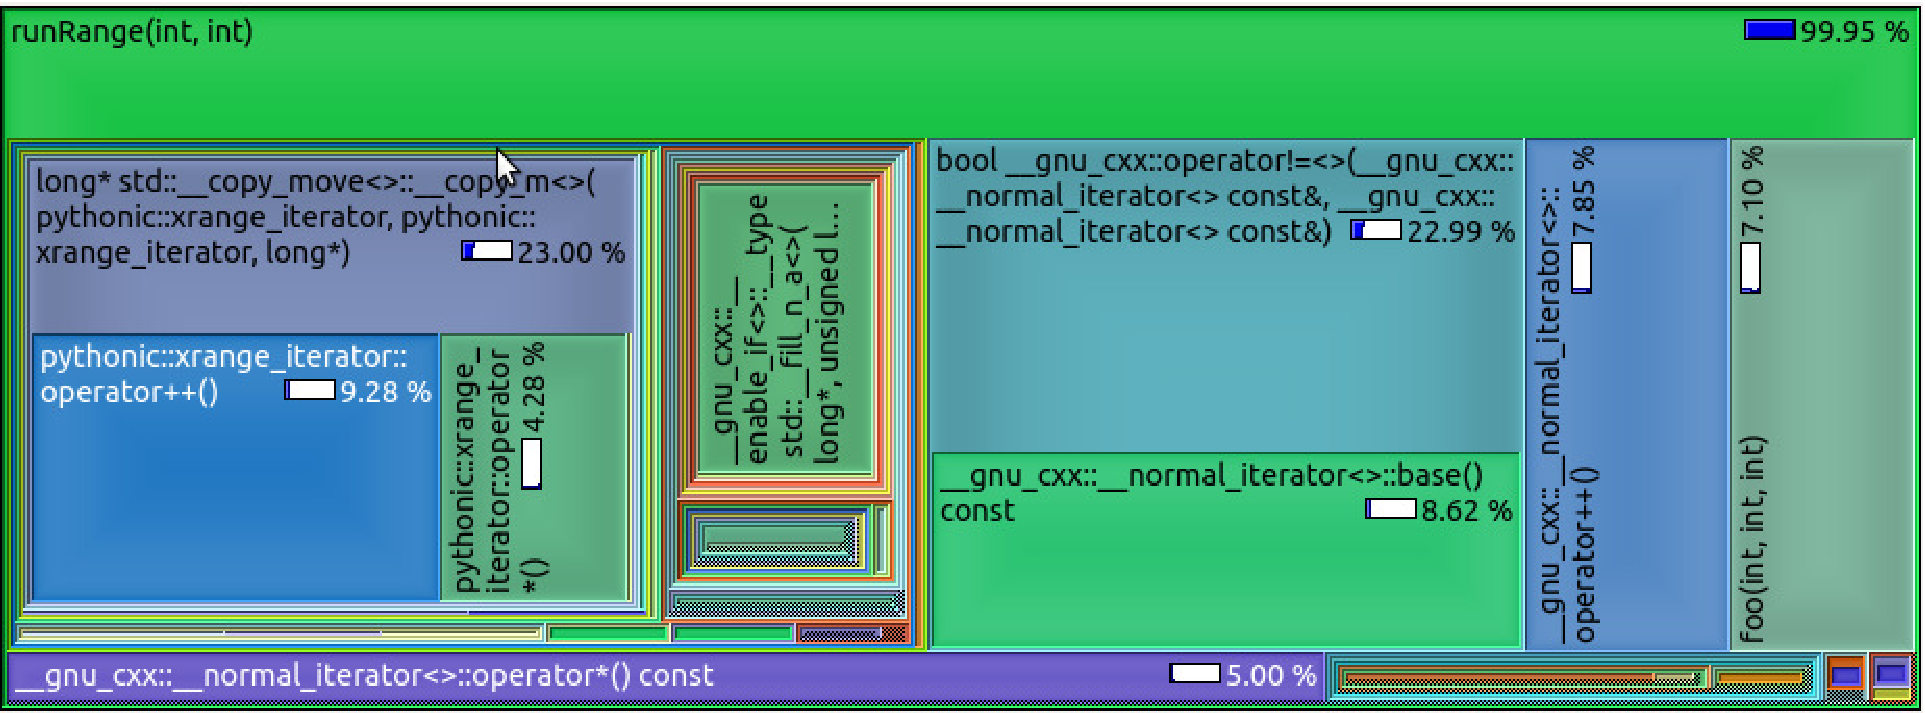
\includegraphics[width=\textwidth]{./Pictures/range}
    \label{pythonvscpp}
  \end{figure}

\end{frame}

%Dans du code en C++, on aurait plutôt fait
%for(int i=0; i < N, i++) --> pas de prob d'alloc de mémoire
\begin{frame}{Conclusion}

  L'allocation/désallocation de mémoire à un prix.

  \pause Dans l'exemple précédent, ce prix n'est pas justifié.

\end{frame}

\section{Réponse à la problématique}

\subsection{Le cas \texttt{xrange}}

\begin{frame}[fragile]
  \frametitle{Principe du \texttt{xrange}}

  \texttt{xrange}:
  \begin{itemize}
    \item Génère $\llbracket 1, n\rrbracket$ élément par élément.  
    \item Est un intrinsèque de python.  
    \item Est implémenté dans pythran.
  
  \end{itemize}

  \pause Exemple :

  \begin{lstlisting}
    for i in xrange(100): 
       print i
  \end{lstlisting}

\end{frame}

% foo = 14% En considerent que foo a dure le meme
% temps que pour le cas range, le code de controle
% a dure plus de deux fois moins longtemps, alors
% que le seule difference est range vs xrange.
\begin{frame}{Résultats}

  \begin{figure}[h]
    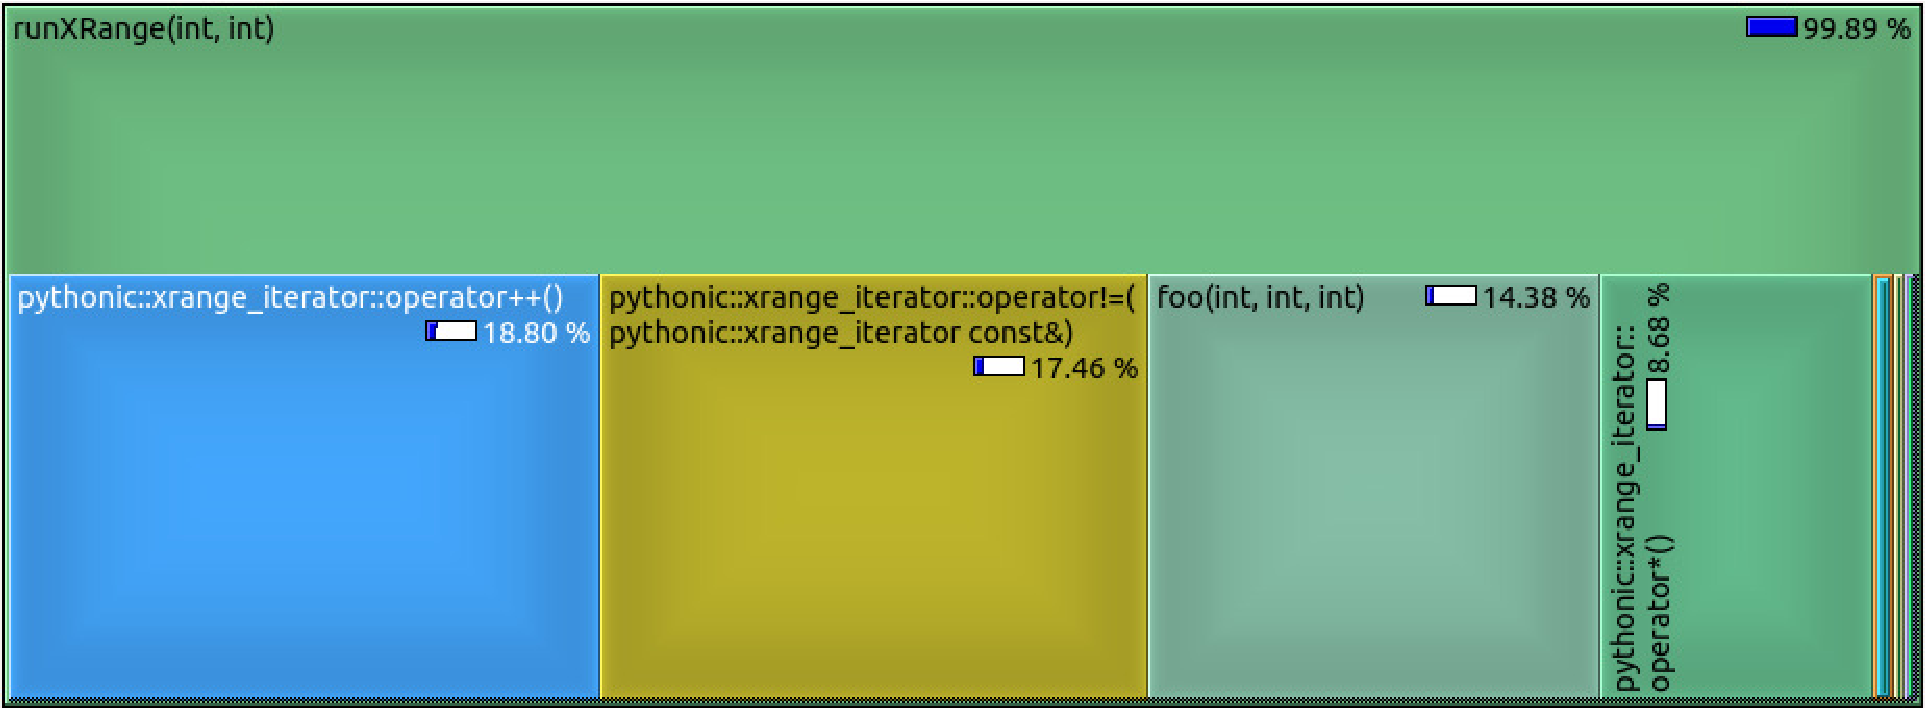
\includegraphics[width=\textwidth]{./Pictures/xrange}
  \end{figure}

\end{frame}

\begin{frame}{Autre test}

  \begin{figure}[h]
    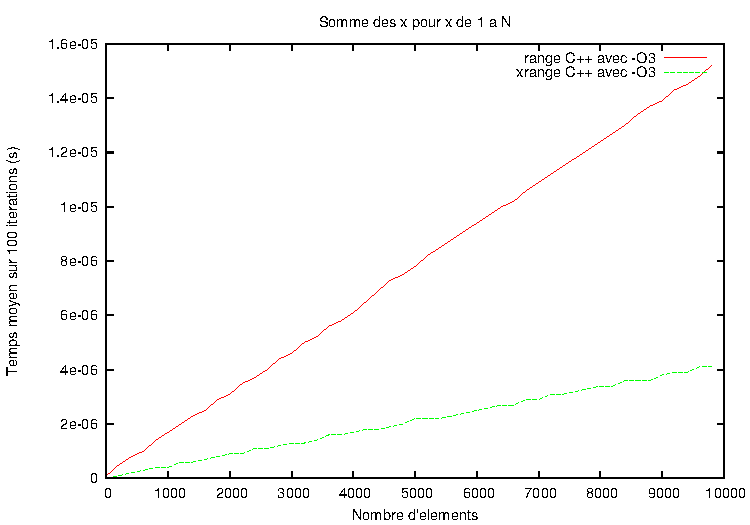
\includegraphics[width=\textwidth]{./Pictures/RangeXrangeCppO3}
    \label{rangexrange}
  \end{figure}

\end{frame}

\begin{frame}[fragile]{Conclusion}

  Remplacer \texttt{range} par \texttt{xrange} peut diviser par 4 le
  temps d'exécution!

  \pause
  \begin{alertblock}{Attention}

    Il existe de nombreux cas dans lesquels remplacer \texttt{range}
    par \texttt{xrange} n'est pas possible.

  \end{alertblock}

  \pause
  Exemple :
  
  \begin{lstlisting}
    l = range(10)
    l[0] = -1
    foo(l)
  \end{lstlisting}


\end{frame}

\subsection{Le module \texttt{itertools}}

\begin{frame}{Le module \texttt{itertools}}

  Le module itertools fournit différents itérateurs remplissant
  diverses fonctions.

  Les itérateurs d'itertools permettent de :

  \begin{itemize}
    \pause \item Ne pas initialiser de mémoire non nécessaire.
    \pause \item De réaliser des séquences infinies.
  \end{itemize}

\end{frame}

\begin{frame}{Contenu}

  Exemples :

  \begin{itemize}
  \item \texttt{imap}, équivalent de \texttt{map}
  \item \texttt{izip}, équivalent de \texttt{zip}
  \item \texttt{product}, produit cartésien
  \item \texttt{permutations}
  \end{itemize}

\end{frame}

\begin{frame}{Résultats attendus}

  \begin{figure}[h]
    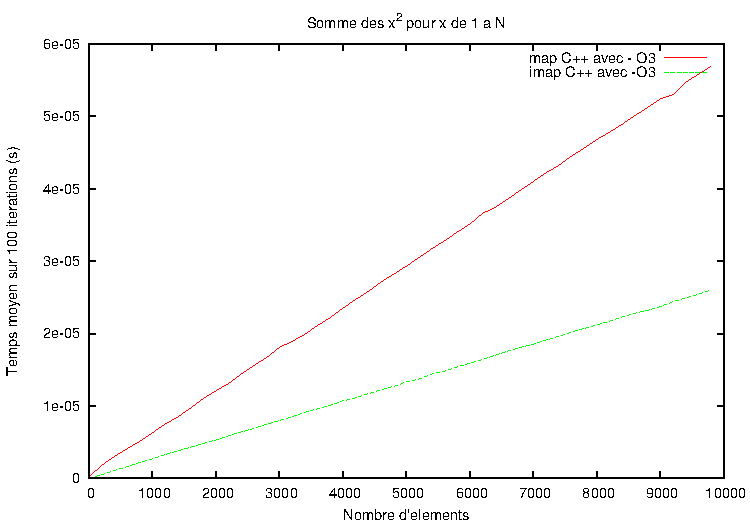
\includegraphics[width=\textwidth]{./Pictures/MapImapCpp}
    \label{mapimap}
  \end{figure}

\end{frame}

\subsection{Transformations de l'AST}

\begin{frame}{Principe}

  AST (Abstract Syntaxic Tree) = Arbre dont les nœuds internes sont
  marqués par des opérateurs et dont les feuilles représentent les
  opérandes de ces opérateurs.

  Le code python est traduit en AST, puis traduit en C++.

  Il est possible d'effectuer des optimisations sur l'AST avant la
  traduction en C++.

\end{frame}

\begin{frame}{Transformations d'itérateurs}

  Principe : Remplacer une fonction créant une liste par un itérateur
  équivalent.

  \pause Exemple :
  \begin{itemize}
  \item \texttt{range} par \texttt{xrange}
  \item \texttt{map} par \texttt{imap}
  \item \texttt{zip} par \texttt{izip}
  \end{itemize}

  \pause \begin{alertblock}{Transformations contextuelles} Il faut
    tout d'abord déterminer si une transformation est valide avant de
    l'appliquer.
  \end{alertblock}

\end{frame}

\begin{frame}{Transformations de \texttt{Generator Expression}}

  Un générateur est un objet de python permettant de générer des
  valeurs.

  Une \texttt{Generator Expression} est une construction de python
  permettant de créer un générateur à la volée.

  \pause\lstinline|( x * x for x in xrange(10) )|

  \pause L'implémentation en C++ n'est pas assez performante. La
  remplacer par l'utilisation d'itérateurs connus devrait améliorer
  les performances.

\end{frame}

\section{Plan de travail}

\subsection{Travail demandé}

\begin{frame}{Implémentation du module \texttt{itertools}}

  Réalisations :
  \begin{itemize}
    \item Implémentation en C++ des itérateurs
    d'\texttt{itertools} 
    \item Intégration à la chaîne de compilation.
  \end{itemize}

\end{frame}

\begin{frame}{Transformations non contextuelles}

  Réalisations :
  \begin{itemize}
    \item Chercher comment exprimer une \texttt{Generator Expression}
    avec des itérateurs.  
    \item Ajouter la transformation à  pythran.
  \end{itemize}

\end{frame}

\begin{frame}{Transformations contextuelles}

  Réalisations :
  \begin{itemize}
    \item Déterminer quels sont les cas dans lesquels il est
    possible d'effectuer les transformations.  
    \item Écrire une analyse en python qui détecte ces cas.  
    \item Ajouter les transformations à pythran.
  \end{itemize}

\end{frame}

\subsection{Méthodes de travail}

\begin{frame}{Travail incrémental}

  Cycle de développement :
  \begin{enumerate}
    \pause \item Définition d'une fonctionnalité à implémenter
    \pause \item Réalisation de cette fonctionnalité 
    \pause \item Validation 
    \pause \item Intégration à pythran.
  \end{enumerate}

\end{frame}

\begin{frame}{Tests unitaires}

  Approche TDD (Test Driven Development) :
  \begin{enumerate}
    \pause \item Écriture des tests que doit passer une fonctionnalité
    \pause \item Réalisation de la fonctionnalités pour réussir les
    tests un à un.  
    \pause \item Pas de régression, tous les autres tests 
    de pythran doivent rester satisfaits.
  \end{enumerate}

\end{frame}

\begin{frame}{Qualité}

  Critères :
  \begin{itemize}
  \item Analyse de la performance des implémentations réalisées
    (valgrind).
  \item Lisibilité du code (PEP8\cite{Pep8}).
  \end{itemize}

\end{frame}

\subsection{Jalons}

\begin{frame}{Présent}

  \begin{itemize}
  \item 23/11 : Rapport court
  \item 21/12 : Présentation orale
  \end{itemize}

\end{frame}

\begin{frame}{À venir}

  \begin{itemize}
  \item 01/02 : Démonstration/Prototype + présentation poster à
    l'ifremer PCIM.
  \item 05/03 : Résumé opérationnel
  \item 11/03 : Restitution
  \end{itemize}

\end{frame}

\section{Conclusion}

\begin{frame}{Références}

  \bibliographystyle{plain}
  \bibliography{presentation}

\end{frame}

\end{document}